\documentclass[11pt]{article}

\usepackage[utf8]{inputenc}
\usepackage[T1]{fontenc}
\usepackage{lmodern}
\usepackage[margin=1in]{geometry}
\usepackage{amsmath}
\usepackage{booktabs}
\usepackage{array}
\newcolumntype{L}[1]{>{\raggedright\arraybackslash}p{#1}}
\usepackage{graphicx}
\usepackage{microtype}
\usepackage{enumitem}
\usepackage[numbers,sort&compress]{natbib}
\usepackage{xcolor}
\usepackage{xurl}
\usepackage[colorlinks=true,linkcolor=blue!50!black,citecolor=blue!50!black,urlcolor=blue!50!black]{hyperref}

\setlist{itemsep=2pt,topsep=4pt}
\newcommand{\pos}[1]{$+#1$}
\newcommand{\nega}[1]{$-#1$}

\title{Loops Look Alive: The Shared Misjudgement\\Behind the Cyclic Attack on Go AIs}
\author{Jaeson Booker\\Independent researcher\\\texttt{jaesonbooker@gmail.com}}
\date{}

\begin{document}
\maketitle

\begin{abstract}
Self-play Go engines that play far above human level lose to a simple ``cyclic'' attack: the adversary builds a closed loop of the victim's stones around its own group and captures the loop. We ask whether this shared blind spot rests on a shared wrong concept inside the networks, where that concept lives, and what adversarial training did to it. We study five networks: a 2020 KataGo self-play net, the net the attack was built against, a post-2023 KataGo trained against the attack, KataGo's human-imitation net and Leela Zero. Using exact labels, freshly generated positions solved by search, published attack games, probes, causal interventions and a small tree search, we find the following. The failure is not in counting liberties but in judging group safety: the vulnerable nets read doomed loops as alive while judging edge groups with the same fate correctly, and the attacked net reads its own lost loops as alive nine times in ten. The mechanism is a ``closed loop'' feature that every net builds by mid-network. In the vulnerable nets it is stored partly as ``safe'', keeps evidence of death from building on the loop, and leaves the final death-detector channels silent. Holding this one direction fixed flips the attacked net's doomed loops from alive to dead. The feature rests on a closure signal that spreads locally and is rebuilt when its channels are removed, and closure means ``alive'' in all three KataGo nets, including the fixed one. Adversarial training did not remove the feature or change what closure means, yet the fixed net reads doomed loops as dead across new loop shapes, without a capturing race, and under an automated search for counterexamples. The vulnerable nets' error survives an 800-visit tree search, and holding the loop direction inside that search reverses its verdict on 11 of 12 doomed loops. For interpretability audits, asking whether a model represents a dangerous feature cannot separate the broken nets from the fixed one. Asking whether the feature drives the decision does.
\end{abstract}

\section{Introduction}

The cyclic attack is a clean case of a superhuman system with a shared, exploitable blind spot. \citet{wang2023adversarial} trained an adversary that beats KataGo, then the strongest public Go engine, by building a loop of the victim's stones around an adversary group and capturing it. Amateur humans can execute the same attack by hand. It transfers to other self-play engines, Leela Zero and ELF among them, which were trained independently with different architectures and inputs.

A blind spot shared across independent training runs matters for AI safety in two ways. If it reflects a shared wrong concept, similar training may produce similar hidden errors elsewhere, and interpretability tools should be able to find them before an adversary does. If instead each engine fails for its own reasons, shared failure says little about shared internals, and audits must be done network by network. We consider three hypotheses for why the engines fail together:
\begin{enumerate}
\item \textbf{Shared wrong concept}: the engines represent the relevant concept, and represent it wrongly in the same way.
\item \textbf{Coverage gap}: the engines lack the concept for these positions because self-play rarely produces them.
\item \textbf{Knowledge not used}: the engines represent the right information but the decision does not use it.
\end{enumerate}

The answer depends on which concept one looks at, and choosing the wrong level gives the wrong answer. At the level of liberty counting, hypothesis 3 fits: the representation is intact. At the level of group safety, hypothesis 1 fits: the vulnerable nets share a wrong judgement, and their play follows it. The adversarially trained net has the same underlying loop feature and a corrected judgement, which is what hypothesis 2 predicts for the fix.

Two further questions follow. The first is whether the mechanism matters for play and not only for readouts. It does: the vulnerable nets' misjudgement survives a tree search, and holding one internal direction during that search reverses the search's verdict (Section~\ref{sec:search}). The second is how good the fix is. We tried to break the fixed net three ways: with new loop shapes, with loops that die without a race, and with an automated search over board edits. It held up in all three once a flaw in our own labels was corrected, and the errors the search did find were shallow enough for a modest tree search to repair (Section~\ref{sec:adv}). We did not find the circuit behind the fix.

Our contributions are:
\begin{itemize}
\item A behavioural test on freshly generated capturing races solved by exact search, which rules out contamination of the public test suite.
\item Evidence that the safety judgement, not liberty counting, is where the self-play nets fail, including in the attacked net on its own lost games.
\item A mechanism, traced from the loop feature through the suppression of death evidence to a few dozen silenced death-detector channels.
\item An account of how the loop feature is built: a local closure signal, computed redundantly, that means ``alive'' in every net we could test.
\item A comparison with the adversarially trained successor, with three attempts to break its fix.
\item Evidence that the misjudgement survives tree search in the vulnerable nets, and a causal test inside the search.
\item A correction to our own generated positions (weak walls), found by the automated search, with the main results re-run on the corrected set.
\end{itemize}

\section{Setup}
\label{sec:setup}

\paragraph{Networks.} Table~\ref{tab:nets} lists the five networks. All are run as raw networks on CPU, with no search except in Sections~\ref{sec:adv} and~\ref{sec:search}.

\begin{table}[h]
\centering\small
\begin{tabular}{@{}L{4.4cm}L{3.6cm}L{3.6cm}L{3.2cm}@{}}
\toprule
Network & Training & Architecture & Role \\
\midrule
g170 (g170e-b20c256x2, 2020) & KataGo self-play & 20-block ResNet, global pooling & vulnerable, pre-attack \\
b40 (kata1-b40c256-s11840935168) & KataGo self-play & 40-block ResNet, global pooling & the net FAR attacked \\
tf3 (kata1-tf3-b11c768) & self-play plus adversarial positions & 11-block conv/attention hybrid & the fixed successor \\
HumanSL (b18c384nbt-humanv0) & imitation of human games (9 dan) & 18-block nested bottleneck & human reference \\
Leela Zero (final 40x256) & independent self-play & 40-block ResNet & second vulnerable family \\
\bottomrule
\end{tabular}
\caption{Networks studied. KataGo is described in \citet{wu2019accelerating}; Leela Zero \citep{leelazero} reimplements AlphaGo Zero \citep{silver2017mastering}. b40 is the net called ``Latest'' (cp505) in \citet{wang2023adversarial}.}
\label{tab:nets}
\end{table}

The KataGo nets receive hand-built input planes that mark chains with 1, 2 or 3 liberties, so any liberty result at those counts is partly given to them. We ran all nets under Japanese rules, where KataGo's area planes are blank, so pass-alive status is not given.

\paragraph{Labels.} Labels are exact and computed from the board, not from any engine: chains, liberties, Benson pass-alive status, eye space and ladders, checked against KataGo's own board code.

\paragraph{Position sets.} All are generated from seeds, so no engine has seen them.
\begin{itemize}
\item \emph{Minimal pairs} (400): a ring enclosing an opponent group, and the same ring cut open by one stone.
\item \emph{Capturing races} (288): a chain racing an enclosed group, walled in so that an exact minimax settles it. There are two geometries with the same liberty counting: a closed \textbf{ring}, and an \textbf{edge} pocket where the board edge closes the enclosure, so no chain encloses anything.
\item \emph{Status sets}: races labelled \textbf{doomed} (the chain is captured if its owner plays elsewhere, but some move saves it) or \textbf{safe}. The \emph{eye-balanced} set (320) gives every inner group exactly one real eye and the ring the same liberty count (5 or 7) in both classes. The \emph{hopeless} set (180) gives the inner group two real eyes, so the ring dies whatever its owner does. The \emph{fortified} set (314) is the eye-balanced set with its opponent walls strengthened (Section~\ref{sec:walls}).
\item \emph{Real games}: FAR's 116 published attack games \citep{wang2023adversarial}, from 1 visit to 10 million visits, including human-played attacks and transfer games, and 2,000 Fox professional games \citep{foxdataset} as a control.
\end{itemize}

\paragraph{Readouts.} The main readout is the \textbf{ownership after a pass}: the chain's owner passes, and the net predicts end-of-game ownership of the chain from the owner's side (\pos{1} lives, \nega{1} dies). This is the label's own counterfactual, read straight off the ownership head. Behaviour is the raw policy's mass on the capturing moves. Internals are read with linear probes per block \citep{alain2016probes} and changed with interventions that hold one direction of the residual stream at a chosen value on the chain's stones \citep{meng2022locating}. Every direction and probe is fit on one half of the positions and tested on the other.

\section{The blind spot, and why liberties are the wrong level}
\label{sec:races}

On fresh races solved by search, the vulnerable nets find the capture against an edge pocket and almost never against a loop (Figure~\ref{fig:races}). The fixed net closes most of the gap.

\begin{figure}[t]
\centering
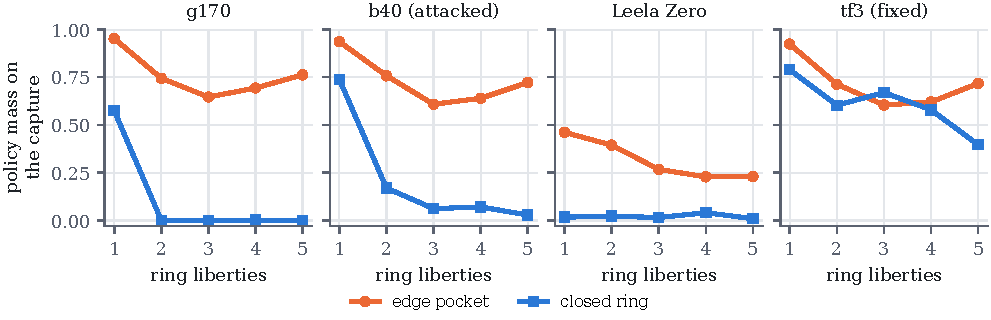
\includegraphics[width=\linewidth]{figures/fig_races.pdf}
\caption{Raw policy mass on the capturing move in 288 generated races, by the racing chain's liberties, for a closed ring and an edge pocket with the same liberty counts. No search.}
\label{fig:races}
\end{figure}

The gap is not a matter of difficulty. At 2 to 5 liberties, g170 puts 0.00 of its policy mass on the capture in ring races and 0.65 to 0.76 in edge races with the same liberty counts. b40 puts 0.03 to 0.07 on it in ring races with 3 to 5 liberties. At 1 liberty, where KataGo is told by an input plane that the chain is in atari, g170 still puts only 0.57 on the capture against a ring (0.95 against an edge). The rest of its mass goes neither to the race nor near the last move, but elsewhere on the board: it plays as if the race were not there.

This also removes a contamination worry. On the public cyclic test positions \citep{goattack}, tf3 puts 0.99 of its policy on the correct answers (g170: 0.04, Leela Zero: 0.16, HumanSL: 0.54). KataGo's anti-cyclic training may include positions like these, but tf3's fix carries over to generated races it cannot have seen (0.62 against 0.70 on edges).

\paragraph{Liberty counting is intact where it should fail.} A linear probe reads each stone's liberty count from each block. On the minimal pairs, closing the loop costs the liberty readout a few points in every self-play net (layer-averaged gap, cut minus cyclic: Leela Zero \pos{0.08}, g170 \pos{0.05}, tf3 \pos{0.05}, HumanSL \pos{0.03}). But on the races, the readout on ring chains is no worse than on edge chains in g170 (\pos{0.01}, 95\% CI $[-0.03, 0.05]$, after adjusting for structure and size), the net with the worst play. It is worst in tf3 (\nega{0.14}), the net with the best play. Within each net, the positions where the readout is worse are not the positions where play is worse (all $|r| < 0.07$). An audit of liberties would clear g170 and flag tf3, backwards on both. Whatever goes wrong sits above liberty counting.

\section{Group safety: loops look alive}
\label{sec:safety}

The vulnerable nets judge a doomed loop to be alive, while judging an edge group with the same fate correctly (Table~\ref{tab:safety}). This is the eye-balanced set: every inner group has exactly one real eye, and the ring has 5 or 7 liberties in both classes, so neither eyes nor the chain's liberty count gives the status away. Leela Zero has no ownership head; its policy captures on 0.01 of doomed rings against 0.16 of doomed edge groups. On an earlier, unbalanced status set the picture is the same (doomed rings: g170 \pos{0.76}, b40 \pos{0.69}, tf3 \nega{0.75}).

\begin{table}[h]
\centering\small
\begin{tabular}{@{}lcccc@{}}
\toprule
Net & Doomed ring & Doomed edge & Safe ring & Capture, doomed ring / edge \\
\midrule
g170 & $\mathbf{+0.99}$ & $-0.33$ & $+0.99$ & 0.00 / 0.55 \\
b40 (attacked) & $\mathbf{+0.66}$ & $-0.51$ & $+0.92$ & 0.03 / 0.51 \\
HumanSL & $+0.55$ & $-0.32$ & $+0.85$ & 0.17 / 0.31 \\
tf3 (fixed) & $\mathbf{-0.68}$ & $-0.55$ & $+0.98$ & 0.52 / 0.54 \\
\bottomrule
\end{tabular}
\caption{Ownership after a pass from the owner's side, eye-balanced set (\pos{1} = lives). Last column: raw policy mass on the capturing moves. On the fortified set (Section~\ref{sec:walls}) the g170 and b40 numbers barely change and tf3 reads doomed rings at \nega{0.86}.}
\label{tab:safety}
\end{table}

Four checks sharpen what the error is.
\begin{itemize}
\item \textbf{It is not only a misread race.} On 180 hopeless loops, where the inner group has two real eyes and the ring cannot be saved, g170 correctly reads the inner group as alive (\nega{0.94} from the ring's side), yet still reads 58\% of the rings as alive too (mean \pos{0.15}; edge groups \nega{0.92}). b40 gets these mostly right (\nega{0.68}). The loop acts as a prior toward life, strong enough to override a close race and, in g170, to leave a hopeless loop half alive.
\item \textbf{In a close race, the enclosed group is read as losing.} In doomed rings the one-eyed inner group actually wins, but g170 reads it as dead (\pos{0.89} from the ring's side) where it reads the same group alive in an edge pocket (\nega{0.52}).
\item \textbf{The judgement forms with depth, later for bigger loops.} A doomed/safe probe trained on edge groups only files doomed rings with doomed edges in the first blocks, then moves every one of them to ``safe'': g170 from block 5, b40 and Leela Zero from block 6, on to the last block. HumanSL moves them and partly brings them back. tf3 pulls them back to ``doomed'' from block 7. On a size-varied set (10 to 60 stones), the block at which g170 flips a doomed ring tracks the ring's size (Spearman 0.87), from blocks 5 to 7 for small rings to 13 to 17 for rings spanning 10 or more points.
\item \textbf{Play follows the judgement.} In tf3, the more doomed it reads a ring, the more it captures ($r = -0.74$, $p < 0.001$). In g170, pushing the ring's stones along the edge-trained ``doomed'' direction at block 3 raises capture on doomed rings about 50-fold (0.003 to 0.16), leaves safe rings and edge groups nearly unchanged, and a random direction does nothing.
\end{itemize}

The self-play nets share a wrong safety concept, located one level above liberties. The human-imitation net partly shares it; the adversarially trained net does not.

\section{Real attack games and the attacked net}
\label{sec:real}

The same judgement shows up where the attack actually happens, and most strongly in the net that was attacked. We took FAR's 116 published attack games and found every chain of 6 or more stones that was captured. For each, we read the positions 1 to 33 moves before the capture, with the losing side to move. 73 of these were victim loops (median 42 stones); 376 ordinary chains from the same games and from 2,000 Fox professional games served as a control. Every chain here did in fact die. 43 of the 73 loop captures are b40's own losses.

\begin{figure}[t]
\centering
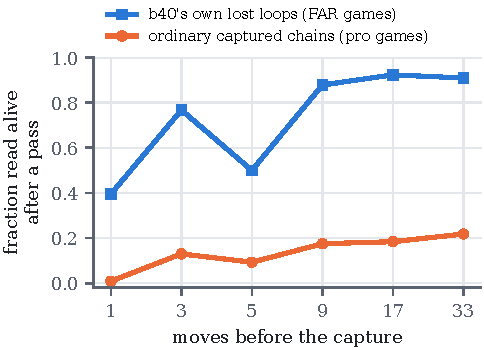
\includegraphics[width=0.6\linewidth]{figures/fig_real.pdf}
\caption{Fraction of chains b40 reads as alive after a pass, by moves before the chain was captured: 43 loop captures from b40's own games in FAR's attack games against 217 ordinary captured chains from professional games. Every chain shown was captured.}
\label{fig:real}
\end{figure}

At 3, 9, 17 and 33 moves before the capture, b40 reads its own lost loops as alive 77\% to 92\% of the time (50\% at 5 moves; Figure~\ref{fig:real}). It reads ordinary chains in the same situation as alive 9\% to 22\% of the time. One move out, with the loop in atari and KataGo's input plane saying so, it still reads 40\% of them as alive. By liberties, b40 reads loops with 3 to 8 liberties at \pos{1.00}, while ordinary chains at 2 to 6 liberties read \nega{0.19} to \nega{0.61}. Adjusted for liberties, chain size and lead time, being a loop shifts the reading by \pos{0.88} (95\% CI $[0.76, 1.00]$) in b40, \pos{0.69} $[0.57, 0.80]$ in g170, \nega{0.04} $[-0.14, 0.08]$ in HumanSL and \nega{0.29} $[-0.66, 0.09]$ in tf3.

Size does not explain it: g170 reads ordinary captured chains of 20 or more stones as dying too (\nega{0.40} to \nega{0.19}, 3 to 9 moves out). The window the attack uses is visible here: the loop is killable for many moves, and the victim spends them elsewhere because it is sure the loop lives.

\section{Mechanism: a loop feature that blocks the evidence of death}
\label{sec:mech}

In the vulnerable nets, a ``closed loop'' feature built by mid-network keeps evidence of death from accumulating on the loop, so the last blocks' death detectors stay silent and the readout says ``alive''. We traced this in five steps, mostly in g170 and b40, whose residual blocks we can decompose exactly.

\subsection{One direction carries the loop}
\label{sec:direction}

For each block, we took the difference between the mean trunk state on ring stones and on edge-group stones, fit on safe positions only, where both geometries get the same verdict. This ``loop direction'' encodes the shape, not the answer: fit on doomed positions instead, it is nearly the same (cosine 0.89 to 0.97). Every net has it, equally strongly. Held-out rings sit 1.7 to 2.0 pooled standard deviations from edge groups along it in g170, b40 and tf3 alike, and a probe on the minimal pairs tells closed from cut loops at 0.95 to 0.99 in all five nets. Holding that one direction (one of 256 dimensions per block) at the edge-group value on the chain's stones removes the error (Table~\ref{tab:holds}). In b40 the doomed-safe gap on rings grows from 0.28 to 0.84 under the hold: once the loop signal is held down, most of the race reading comes back.

\begin{table}[h]
\centering\small
\begin{tabular}{@{}lccc@{}}
\toprule
Net, blocks held & Doomed ring: ownership / capture & Safe ring & Doomed edge \\
\midrule
g170, none & $+0.99$ / 0.00 & $+0.99$ & $-0.26$ \\
g170, 6--12 & $\mathbf{+0.26}$ / \textbf{0.14} & $+0.65$ & $-0.10$ \\
b40, none & $+0.65$ / 0.04 & $+0.93$ & $-0.51$ \\
b40, 12--24 & $\mathbf{-0.23}$ / \textbf{0.26} & $+0.61$ & $-0.46$ \\
random directions, same blocks & no change & no change & no change \\
\bottomrule
\end{tabular}
\caption{Holding the loop direction at the edge-group level on the chain's stones, held-out half of the eye-balanced set.}
\label{tab:holds}
\end{table}

\subsection{The error is made where the verdict is written}

A doomed/safe probe first moves rings to ``safe'' at blocks 3 to 5 in g170, but holding or patching there changes nothing. The causal window is later. We decomposed each block's update along the final verdict axis (the direction from doomed to safe edge groups at the last layer). The loop-specific push onto the verdict is written almost entirely at the end: the last block writes \pos{0.53} of g170's final position of doomed loops (\pos{0.99} in total) and \pos{0.36} of b40's (\pos{0.63}). The last quarter of each net writes \pos{0.87} and \pos{0.58}. For safe rings the same late writes are near zero, so the push appears exactly when the race says the loop dies. Removing it at b40's blocks 28 to 40 makes doomed loops read \nega{0.48}, the same as doomed edge groups (\nega{0.49}), with safe loops still at \pos{0.98}.

\subsection{The late push is a silenced death detector}

Splitting the last blocks' writes over their 256 hidden channels, 27 of b40's top 32 contributors (29 of 32 in g170) are ``this group is dying'' channels. They fire on doomed edge groups and stay near silent on doomed loops and on safe groups (b40 block 40, channel 102: 10.3 on doomed edges, 0.3 on doomed loops, 0.0 on safe groups). Across the top 16, doomed loops get 20\% of the doomed-edge activation in b40 and 10\% in g170. Zeroing the top 32 makes doomed edge groups read alive (b40: \nega{0.51} to \pos{0.89}); 32 random channels do nothing. Setting 16 of them on doomed loops to the level doomed edges get moves b40's doomed loops from \pos{0.65} to \pos{0.27}, with safe loops barely changed.

\subsection{The loop feature keeps them silent, during mid-network}

Holding the loop direction at blocks 12 to 24 in b40 re-lights the death channels on doomed loops (from 20\% to 59\% of the doomed-edge level, twice what safe loops get). Holding it only just before the last blocks does nothing. Death evidence, measured on each layer's axis from safe to doomed edge groups (safe edge = 0, doomed edge = 1), shows why. On doomed loops it starts near 0.7, then falls \emph{below} safe edge groups through b40's blocks 10 to 22 (\nega{0.1} to \nega{0.5}). A global-pooling block (26) lifts every ring toward ``dying'' (doomed loops to 1.12), but blocks 27 to 40 erode it again to 0.41.

In b40, holding the loop direction at any single block from 12 to 23 lowers doomed loops to \pos{0.14} to \pos{0.30}. At block 24 it does nothing (\pos{0.60}). After a single hold at block 12 the loop feature grows back completely by block 26, yet the loop still reads less alive: death evidence written in the gap is not erased. g170 rebuilds the feature within about four blocks, so only multi-block holds work there (blocks 10 to 12: \pos{0.51}).

\subsection{Why: the loop is stored partly as ``safe''}

In mid-network, the loop direction and the death direction point partly against each other: cosine \nega{0.28} to \nega{0.43} in g170 (blocks 6 to 11) and \nega{0.17} to \nega{0.36} in b40 (blocks 10 to 22). The vulnerable nets encode ``this chain is a loop'' in a subspace that also means ``this chain is safe''. So the loop feature is itself evidence against death, and pushes the chain off the death side while the race is being read.

\section{How the loop feature is built}
\label{sec:closure}

\subsection{A local closure wave}

The minimal pairs isolate closure: the cyclic and cut members differ at one point, so anything that depends on the ring being closed must start at the cut and spread. After removing two input leaks (Section~\ref{sec:limits}), 131 pairs remain. The closure signal spreads outward from the cut by local propagation through the convolutions. Far ring stones (8 to 12 steps from the cut) go from 0.01 standard deviations at the stem to 0.94 at layer 5 and 1.55 at layer 7 in g170, and more slowly in b40 (0.47 and 0.77). In g170 it reaches every distance before the first global-pooling block. It travels by board distance, not along the chain: the signal falls 0.09 to 0.19 SD per point of board distance and 0 to 0.08 per step along the ring.

Part of it goes through the enclosed region. Overwriting the interior with the cut member's states removes 35\% to 43\% of the closure signal at far ring stones, and overwriting a band outside the ring removes 5\% to 10\%. The net computes closure partly as a property of the region: sealed off from the outside, and felt by the stones that bound it.

This closure signal is a component of the loop direction exactly in the causal windows (cosine 0.35 to 0.48 in g170's blocks 7 to 12, 0.27 to 0.39 in b40's 11 to 18, near 0 at the input layers). Holding the pure closure direction, taken from the minimal pairs and so free of edge geometry, at b40's blocks 12 to 24 moves doomed loops from \pos{0.65} to \pos{0.25} and raises capture from 0.04 to 0.15, with random directions doing nothing. That is about half the effect of the full ring-minus-edge direction. In g170 the same hold barely moves the verdict (\pos{0.99} to \pos{0.91}).

\subsection{Closure is redundant, and tf3 computes it at once}

The closure wave has no small circuit. Each block's write along the closure direction splits exactly over its hidden channels, because the block's final convolution is linear. Across blocks 1 to 12, 128 of 2,944 channels carry half of the positive write in g170, and 119 in b40. Some channels specialise on the enclosed region: the interior is 3\% of the board but holds 20\% to 32\% of these channels' cyclic-minus-cut difference, and three of g170's top block-5 channels put 83\% to 99\% of it inside the ring.

Removing those channels does not remove closure. Setting the top 512 channels in blocks 1 to 12 to the cut member's values cuts the closure signal at block 12 to 0.29 of baseline in g170 and 0.22 in b40. Four to twelve blocks later it is back at 0.74 and 0.89, and the ownership difference between cyclic and cut members does not move (0.95 and 1.01 of baseline). The later blocks recompute closure from what remains, so channel ablation is the wrong tool here and direction holds on the trunk are the right one. The loop feature regrew after mid-trunk holds for the same reason.

The two convolutional nets use closure differently. In g170, holding the closure direction does nothing in blocks 6 to 12. In blocks 13 to 16 it moves doomed rings to \pos{0.49}, but safe rings and safe edge groups both fall to \pos{0.62}: by then g170's closure direction lies along a general life axis rather than a ring-specific one. In b40 (blocks 12 to 24) the hold moves doomed rings by \nega{0.40}, safe rings by \nega{0.23}, and safe edge groups by only \nega{0.05}. In the attacked net closure is a ring-specific input to the verdict; in g170 it is not a separate lever at all.

tf3 builds closure differently from both. Every ring stone gets half its peak closure signal by block 1 or 2, against layers 2 to 9 in the convolutional nets. From block 4 on, the signal grows with distance from the cut along the chain (\pos{0.09} to \pos{0.18} SD per step) and falls with board distance, the opposite of the local wave. Points outside the ring get nothing. tf3 computes closure as a property of the whole chain, through attention.

\subsection{Closure means ``alive'' in all three nets}
\label{sec:closurealive}

In every net the closure direction points away from death. Its cosine with the death axis (safe edge to doomed edge) is \nega{0.57} to \nega{0.75} in g170's blocks 6 to 12, \nega{0.81} to \nega{0.88} in b40's last 15 blocks, and \nega{0.62} to \nega{0.78} in tf3 from block 3 on. What differs is how far death pulls rings down along this life axis. In the last third of each net, doomed edge groups sit about 2 SD below safe ones everywhere. Doomed rings sit 0.06 to 0.36 SD below safe rings in g170, 0.55 to 0.77 in b40, and 1.31 to 1.80 in tf3. That order matches the verdicts on doomed rings: \pos{0.99}, \pos{0.66} and \nega{0.65}.

Injected closure revives a doomed group in all three nets. On the chain's stones, we set the closure component to the level of the other geometry with the same status, so edge groups get a ring's closure and rings get an edge group's. Doomed edge groups go from dead to alive: \nega{0.25} to \pos{0.96} in g170, \nega{0.49} to \pos{0.23} in b40, and \nega{0.43} to \pos{0.68} in tf3. The capture move falls from about half the policy mass to 0.00, 0.13 and 0.08. Random directions with the same targets change nothing. Taking closure away from rings does little in any net, as expected from its redundancy.

So adversarial training did not change what closure means to tf3. Closure is still sufficient evidence of life, and the level that tf3's doomed rings reach would revive an edge group. What tf3 has is death evidence on doomed rings strong enough to override it.

\section{What adversarial training changed}
\label{sec:adv}

tf3 kept the loop feature and changed how it feeds the safety judgement (Table~\ref{tab:compare}). Three things stand out. First, the representation of the dangerous shape is intact: tf3 recognises closed loops as clearly as the broken nets, and even shows the same early ``looks alive'' bump. Second, from block 6 on, tf3 stores the loop on the ``dangerous'' side of the safety subspace (cosine \pos{0.24} to \pos{0.36}), where the broken nets store it on the ``safe'' side. The flip is not in closure itself, which still means ``alive'' in tf3, but in the rest of the ring's geometry. Third, the verdict no longer depends on the feature: holding tf3's loop direction at the edge value changes its verdict on doomed loops by 0.01, and its last blocks write no loop-specific push to remove. Its safety reading predicts its play position by position ($r = -0.74$).

This resolves an earlier puzzle. tf3 fixed its play on loops but kept, and even worsened, the degraded liberty readout on closed loops (Section~\ref{sec:races}). Adversarial training did not repair the low-level representation, nor remove the loop feature.

\begin{table}[h]
\centering\small
\begin{tabular}{@{}lccc@{}}
\toprule
 & g170 & b40 (attacked) & tf3 (fixed) \\
\midrule
Loop feature present (rings from edges, pooled SDs) & 1.7--2.0 & 1.7--2.0 & 1.7--2.0 \\
Closed vs cut loop decodable (minimal pairs) & 0.99 & 0.99 & 0.99 \\
Cosine of loop and death directions, mid-network & $-0.28$ to $-0.43$ & $-0.17$ to $-0.36$ & $\mathbf{+0.24}$ \textbf{to} $\mathbf{+0.36}$ \\
Cosine of closure and death directions & $-0.57$ to $-0.75$ & $-0.81$ to $-0.88$ & $-0.62$ to $-0.78$ \\
Late loop-specific push toward ``alive'' & $+0.87$ & $+0.58$ & $\mathbf{-0.15}$ \\
Holding the loop direction: doomed ring ownership & $+0.99 \to +0.26$ & $+0.65 \to -0.23$ & $\mathbf{-0.73 \to -0.72}$ \\
Doomed ring ownership, no intervention & $+0.99$ & $+0.65$ & $-0.68$ \\
Capture on doomed rings & 0.00 & 0.03 & 0.52 \\
\bottomrule
\end{tabular}
\caption{The mechanism in the vulnerable nets and the fixed one, eye-balanced set.}
\label{tab:compare}
\end{table}

\subsection{Three attempts to break the fix}

\paragraph{New loop shapes.} If tf3's extra death evidence were tied to the shape of the loops it was trained against, a doomed loop with a new shape should fool it. We built 150 fresh races with exact labels, 20 doomed and 10 safe per shape: the standard thin ring, a ring two stones thick, a ring with an arm sticking out, a ring along the first line, and a big ring of 26 to 40 stones. tf3 reads doomed loops as dead in every shape (\nega{0.58} standard, \nega{0.88} thick, \nega{0.60} with an arm, \nega{0.71} on the first line, \nega{0.62} big), with capture mass 0.37 to 0.50. g170 reads every doomed loop alive (\pos{0.99} to \pos{1.00}), and b40 does too (\pos{0.64} to \pos{0.91}, worst on big loops). Safe loops read alive everywhere. The non-closure part of tf3's loop direction does not carry the counterweight on its own: holding it over blocks 3 to 9 cuts tf3's capture mass on doomed rings from 0.52 to 0.29 but moves ownership only from \nega{0.65} to \nega{0.54}.

\paragraph{Loops that die without a race.} What the five shapes share is the race: an enclosed opponent group with an eye, a few shared liberties, a surrounded chain. If tf3 had learned to read that race, loops that die without one should fool it. They do not. On the hopeless set, tf3 reads all 90 loops as dead (\nega{0.97}), more firmly than the matched edge groups (\nega{0.92}). The same test narrows the attacked net's blind spot: b40 reads hopeless loops as dead (\nega{0.68}, 3\% alive) but race loops as alive (\pos{0.66}, all of them). Its error is specific to loops in a capturing race, which is exactly what the cyclic attack sets up. g170 fails on both.

\paragraph{An automated search.} \label{sec:walls}
We searched for doomed loops that tf3 reads as alive. Starting from doomed loops, we changed one to three points at a time, mostly within three points of the race, and kept a change only if the position was still a closed race that the owner loses after a pass, solved exactly. A beam search per position (width 3, 12 mutants per parent, 10 steps) kept the changes that raised tf3's ownership of the loop.

The first search flipped tf3 within 8 to 10 changed points, by placing stones against the opponent walls that seal the ring's outside liberties. Those walls turned out to be weak in every generated position: some wall chain always had fewer liberties than the ring. Our race solver never lets the ring's owner capture a wall stone. A stricter solver that does showed the first flipped position was savable. tf3 was right and our label was wrong. We therefore fortified the walls, adding opponent stones until every wall chain had at least the ring's liberties plus two, and re-solved; 314 of 320 positions kept their status. The main contrasts hold and sharpen. g170 and b40 still read every doomed ring alive (\pos{0.99} and \pos{0.58}), against \nega{0.62} and \nega{0.71} for doomed edge groups. tf3 reads doomed rings as dead (\nega{0.86}) and gets 1\% wrong instead of 11\%: most of its apparent errors had been positions where a weak wall gave the loop real chances.

With strong walls, tf3 resists. Searching from 20 fortified doomed loops, with every mutant required to keep its walls strong, pushed 3 of 17 above zero and 1 above \pos{0.5}, after 13 to 20 changed points. In that one, tf3's ownership reaches \pos{0.66} and its policy on the saving capture falls from 0.79 to 0.002. 14 of 17 loops stayed dead through ten rounds of selection. These finds rest on our solver's assumption that a wall with two liberties more than the ring cannot be profitably attacked.

Section~\ref{sec:search} shows that a modest tree search corrects all three. tf3's fix depends on neither the loop's shape, nor a race, nor any single direction we could hold. The simplest reading left is that tf3 weighs the ordinary evidence of a surrounded chain at full strength on loops, where the older nets let closure mute it. We have not found the circuit that does this.

\section{The blind spot under search}
\label{sec:search}

KataGo's own engine was not available in our environment, so we wrote a small PUCT search that uses each network's policy, value, score and ownership heads: 800 visits, all legal moves with prior at least $10^{-5}$, batches of 8 leaves with virtual loss, and a utility of win/loss plus a dynamic score term in the style of KataGo. The score term matters: the random board around our races leaves the loop's owner lost overall, and with win/loss alone the search had nothing to prefer. Ownership under search is the visit-weighted average of leaf ownership. Each network searches with itself.

\paragraph{The vulnerable nets stay blind.} On 12 doomed rings from the fortified set, with 4 doomed edge groups and 4 safe rings as controls, g170 and b40 still read every doomed ring as alive after the owner passes (\pos{0.98} and \pos{0.78}, against \pos{0.99} and \pos{0.55} raw; b40 gets worse). With the owner to move they put almost no visits on the capture that saves the ring (0.00 and 0.03). On edge groups the same networks with the same search put 99\% to 100\% of visits on it and read the group as dead after a pass (\nega{0.86} and \nega{0.93}). Safe rings stay alive (\pos{0.99} and \pos{0.92}). tf3 reads the 12 rings as dead before and after search (\nega{0.90} and \nega{0.85}) and finds the saving capture with 87\% of visits. After the pass it is the same network playing the attacker, and the vulnerable nets do not find the kill either. This matches FAR's games, where the victim does not defend a loop its own search believes is safe. The ownership and value heads say ``alive'' at every node the search visits near the loop, and the policy gives the capture little prior (0.00 and 0.08), so the error is in the evaluation, not in a missing variation.

\begin{figure}[t]
\centering
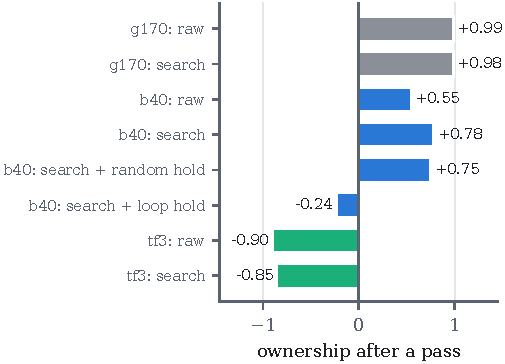
\includegraphics[width=0.62\linewidth]{figures/fig_search.pdf}
\caption{Ownership of 12 doomed rings after the owner passes (\pos{1} = alive), fortified set: raw network, 800-visit search, and for b40 the same search with the loop direction (or random directions) held at the doomed-edge level on the ring's stones in blocks 12 to 24 at every evaluated node.}
\label{fig:search}
\end{figure}

\paragraph{The same direction blinds the search.} We ran the intervention of Section~\ref{sec:direction} inside the search. At every node b40 evaluates, the loop direction is held at the doomed-edge level over blocks 12 to 24 on the ring's stones still on the board, with the direction and target switching with the side to move. With the hold, b40's search reads 11 of 12 doomed rings as dead after a pass (mean \nega{0.24}, from \pos{0.78}; Figure~\ref{fig:search}). Random directions change nothing (\pos{0.75}, all 12 alive). Visits on the saving capture rise from 0.03 to 0.23: it becomes the majority choice in 2 of 12 positions and passes a quarter of the visits in 3, where no position passed 0.06 without the hold. Nine of the 12 rings lie outside the half the direction was fit on, and give the same numbers. The hold is not a repair: safe rings fall from \pos{0.92} to \pos{0.38} and one of four reads as dead, because it removes a loop's protection whether or not the loop deserves it.

\paragraph{tf3's constructed errors are shallow.} On the three positions the automated search flipped, 800 visits take the loop from alive (\pos{0.38}, \pos{0.43}, \pos{0.66} raw) to dead (\nega{0.78}, \nega{0.74}, \nega{0.76}) after the owner passes, and on their unflipped originals the search is correct throughout. One failure of a different kind remains: in the strongest position, with the owner to move, the search never visits either saving capture (raw priors 0.0016 and 0.0006). It no longer believes the loop is safe (ownership \nega{0.31}); it believes the loop is dying and does not see the save. This search is tf3 judging its own positions, so it corroborates our labels but does not prove them.

\section{Implications for interpretability audits}
\label{sec:audit}

Three audits of the same three networks give three different answers, and only one matches behaviour (Table~\ref{tab:audit}).

\begin{table}[h]
\centering\small
\begin{tabular}{@{}L{5.6cm}cccL{3.6cm}@{}}
\toprule
Audit question & g170 & b40 & tf3 & Matches behaviour? \\
\midrule
Is the low-level concept (liberties) intact on loops? & yes & not tested & worst & \textbf{no}: ranks them backwards \\
Is the dangerous feature (a closed loop) represented? & yes & yes & yes & \textbf{no}: cannot tell them apart \\
Does that feature drive the safety decision? & yes & yes & no & \textbf{yes} \\
\bottomrule
\end{tabular}
\caption{Three audits of the same networks. Only the causal question separates the vulnerable nets from the fixed one.}
\label{tab:audit}
\end{table}

\paragraph{Audit the concept the decision uses, not the obvious one.} The capture decision depends on a safety judgement, not on a liberty count. A liberty audit, the natural first check for a capturing race, clears the vulnerable net and flags the fixed one.

\paragraph{Representation is not use.} Finding that a model represents a dangerous feature says little about risk. All three nets represent loops equally well. What differs is whether that representation feeds the decision, and in which direction. A causal test, holding the feature fixed and watching the output, separates them, and the same test changes what the engine does under search. So does a cheap geometric check: the sign of the feature's projection on the decision's own axis.

\paragraph{Fixes can be local and invisible to representational audits.} Adversarial training changed how a feature is used and left its representation, and a related low-level representation, as they were or worse. A post-fix audit that looks for the feature would conclude nothing changed; one that looks at play alone cannot say why it changed or whether it generalises. Here it does generalise, to fresh positions, new shapes, real games and an automated search.

\paragraph{Shared blind spots can come from shared shortcuts.} In two generations of KataGo, the shape ``closed loop'' became partly synonymous with ``safe'', and Leela Zero's safety probe shows the same drift of doomed loops to ``safe''. A plausible reason is that in self-play, large connected loops are nearly always alive, so the shortcut is almost always right. That is the sense in which the failure is a shared wrong concept: a useful correlation promoted into the safety judgement.

\paragraph{Adversarial tests can audit the auditor.} Our automated search first ``fooled'' the fixed net by exploiting a flaw in our own labels. Searching for a model's errors also searches for the evaluator's, and a hit needs an independent check before it counts against the model.

\section{Limitations}
\label{sec:limits}

\begin{itemize}
\item \textbf{Limited search.} Most readouts are the raw network. Our search tests use a simplified PUCT search of our own at 800 visits, with each network judging its own positions, on 12 rings per network. FAR's games were played with up to 10 million visits. We did not run KataGo's own engine.
\item \textbf{Synthetic positions.} The races are walled-in, artificial positions with a random board around them. The real-game results agree, but the mechanism was traced on the synthetic sets. Their opponent walls were weak, which made some doomed labels wrong; fortifying the walls leaves the g170 and b40 results unchanged and cuts tf3's error rate from 11\% to 1\%. The fortified labels still assume that a wall with two liberties more than the ring cannot be profitably attacked.
\item \textbf{Directions are mean differences.} The loop direction, verdict axis and death axis are one averaged direction per layer. They may carry more than their names (ring stones sit mid-board, edge stones near the edge). Fitting on safe positions rules out the verdict itself, not every geometric confound. The pure closure direction answers this for b40, but explains little of g170's error.
\item \textbf{Label-assisted interventions.} Restoring death channels and removing late verdict writes use the true status to pick the reference level. They show where the loop-specific component enters and that these channels suffice, not that the net could recover status unaided. The direction holds use the same doomed-edge target for every position.
\item \textbf{Channel analysis on ResNets only.} tf3 mixes attention and convolution, and we did not decompose its blocks; its contrast rests on direction-level tests.
\item \textbf{Stand-in versus victim.} The mechanism was found in g170 first, then confirmed in b40. Leela Zero and ELF, also vulnerable, were not traced beyond probes.
\item \textbf{Input leaks.} Under territory scoring, KataGo's feature code shifts the komi input by the difference in stones each side has placed, and the ladder planes are computed chain-wide. Both vary with the random board around our positions. We removed them for the closure analysis; elsewhere they are nuisance inputs, not tied to status or geometry.
\item \textbf{The shortcut story is a hypothesis.} We did not measure how often loops live in self-play data.
\item \textbf{Small samples in places.} Several of the later tests use 12 to 30 positions per cell; we report them with their counts.
\end{itemize}

\section{Related work}
\label{sec:related}

\paragraph{Adversarial policies in Go.} \citet{wang2023adversarial} found the cyclic attack and showed it transfers across engines and can be executed by humans. \citet{tseng2025robust} tested defences, including KataGo's adversarial training, and found that new adversaries still win. We use their published games and the attacked net, and ask what inside the networks the attack exploits.

\paragraph{Concepts in game-playing networks.} \citet{mcgrath2022acquisition} probed AlphaZero for human chess concepts layer by layer, and \citet{schut2025bridging} discovered concepts in AlphaZero beyond human knowledge. We use the same probing idea, but on a known failure, with exact labels and causal tests, and compare networks that fail with one that was fixed.

\paragraph{Probing and causal interventions.} Linear probes follow \citet{alain2016probes}. Holding a direction at a reference value and patching activations follow the causal-tracing line of work \citep{meng2022locating}. The contrast between ``represented'' and ``used'' is the central methodological point of that literature, applied here to an audit and carried into play under search.

\section*{Code and data availability}

All code, generated position sets and result files are at \url{https://github.com/jaebooker/go-concepts}; its build log (\texttt{docs/build-log.md}) records each experiment with the exact numbers quoted here. Everything runs on CPU. Networks: g170e-b20c256x2 and b18c384nbt-humanv0 from KataGo's GitHub releases; kata1-b40c256-s11840935168-d2898845681 and kata1-tf3-b11c768-s11001M-d5973M from \url{https://katagotraining.org}; Leela Zero's final 40x256 network. g170 and b40 are loaded from KataGo's \texttt{.bin.gz} format by our own loader, checked by full parse and policy agreement with professional moves. On our CPU, tf3's PyTorch forward pass ran about 40 times slower than it should because of denormal floating-point values; flushing them to zero (\texttt{torch.set\_flush\_denormal(True)}) gives identical outputs.

\section*{Acknowledgments}

Claude (Anthropic) was used extensively for writing code, running experiments and drafting this paper. The author directed the research and is responsible for its content. We thank FAR AI for publishing their attack games and code, and the KataGo and Leela Zero projects for their public networks.

\bibliographystyle{plainnat}
\bibliography{refs}

\appendix
\section{Experiment map}

\begin{table}[h]
\centering\scriptsize
\begin{tabular}{@{}L{4.2cm}L{5.6cm}L{5.6cm}@{}}
\toprule
Result & Module & Output \\
\midrule
Exact labels & \texttt{labels.py}, \texttt{tests/test\_labels.py} & 7 tests \\
Minimal pairs, liberty probes (\S\ref{sec:races}) & \texttt{cyclegen.py}, \texttt{pairs\_eval.py}, \texttt{pairs\_layeravg.py} & \texttt{runs/pairs\_layeravg\_m60.json} \\
Solved races (\S\ref{sec:races}) & \texttt{racegen.py}, \texttt{race\_eval.py} & \texttt{runs/races\_report.json} \\
Status sets (\S\ref{sec:safety}) & \texttt{statusgen.py}, \texttt{status\_eval.py}, \texttt{hopeless\_eval.py} & \texttt{runs/statusbal\_report.json} \\
Real attack games (\S\ref{sec:real}) & \texttt{realgames.py} & \texttt{runs/real\_report.json} \\
Loop direction holds (\S\ref{sec:direction}) & \texttt{mech.py}, \texttt{mech\_cross.py} & \texttt{runs/mech\_cross\_*.json} \\
Verdict path, death channels, gating (\S\ref{sec:mech}) & \texttt{verdict\_path.py}, \texttt{late\_channels*.py}, \texttt{gating.py} & \texttt{runs/verdict\_*}, \texttt{runs/late\_channels*}, \texttt{runs/gating\_*} \\
Closure wave and channels (\S\ref{sec:closure}) & \texttt{loopcircuit.py}, \texttt{closure\_channels.py}, \texttt{closure\_hold.py} & \texttt{runs/loopcircuit\_*}, \texttt{runs/closure\_*} \\
Closure as life (\S\ref{sec:closurealive}) & \texttt{tf3\_closure.py}, \texttt{closure\_swap.py} & \texttt{runs/tf3\_closure\_*}, \texttt{runs/closure\_swap\_*} \\
New shapes, hopeless loops (\S\ref{sec:adv}) & \texttt{shapegen.py}, \texttt{shape\_eval.py}, \texttt{tf3\_counterweight.py} & \texttt{runs/shapes\_*}, \texttt{runs/*/hopeless.json} \\
Automated search, fortified walls (\S\ref{sec:adv}) & \texttt{attack\_search.py}, \texttt{race\_ext.py}, \texttt{fortified\_set.py} & \texttt{runs/attack\_flip.json}, \texttt{runs/status\_bal\_fortified\_*} \\
Tree search, holds in search (\S\ref{sec:search}) & \texttt{mcts.py} & \texttt{runs/mcts\_*} \\
\bottomrule
\end{tabular}
\end{table}

\end{document}
